\documentclass{sysuthesis}

%%
% 论文相关信息
% 本文档中前缀"c-"代表中文版字段, 前缀"e-"代表英文版字段
% modifyer: 黄俊杰(huangjj27, 349373001dc@gmail.com)
% update date: 2017-04-13
%%

% 标题
% 论文题目应以简短、明确的词语恰当概括整个论文的核心内容,避免使用不常见的缩略词、缩写字。读者通过标题可大致了解毕业设计(论文)的内容、专业的特点和科学的范畴。中文题目一般不宜超过 24 个字,必要时可增加副标题。外文题目一般不宜超过 12 个实词

% 封面标题。由于技术所限,封面题目过长的划分交由用户您进行定夺
% 这也能让您的论文封面看起来更有美感
\covertitlefirst{基于Angular框架的}
\covertitlesecond{产品及资源包管理web应用}

% 另外一种封面的论文题目. 换行使用换行符("\\")
%\title{
%    中山大学 \\
%    本科毕业论文非正式模版
%}

% 中英文标题
\ctitle{基于Angular框架的产品版本及资源包管理web应用}
\etitle{
	A web application based on Angular frame 
		to manage packages
}

% 作者详细信息
\author{刘发斌}
\cauthor{刘\ 发\ 斌}    % 封面作者
\eauthor{Liu Fabin}
\studentid{14353196}
\cschool{数据科学与计算机学院}

\cmajor{软件工程(移动信息工程)}
\emajor{Software Engineering}

% 指导老师
\cmentor{王变琴\ (高级工程师)}
\ementor{SN ENGR. Wang Bianqin}

     % 论文相关信息
%%
% 开题报告
% modifier: 黄俊杰(huangjj27, 349373001dc@gmail.com)
% update date: 2017-05-14

% 选题目的
\objective{
时代在进步,技术在发展,我们需要改变自己的观念,在摸索中不断尝试新的事物。
本论文基于企业的产品线控制的需求,致力于建立一个完善的资源包管理应用,为产品版本的开发,测试,审核,发布等流程的管理提出的一站式解决方案。
技术实现上,本应用基于目前较成熟的angular框架,实现资源包控制线的一系列功能,在实践中发掘目前前端技术上的优缺点,改变前端的思维模式。
}

% 思路
\methodology{
该应用需要包括三方面的功能:

账户管理的功能包括登录,注册,注销,更改个人信息,基本满足了对于应用使用者的需求
产品管理的功能包括修改产品信息,添加某角色(产品开发者/测试员)的成员,删除某角色的成员,更换管理员,新建产品(即提交新产品的信息和新建产品的第一个版本)。
版本管理的功能包括新建版本(需要上传新版本的资源包),版本流程的管理(测试,审核,发布),版本回滚。
最后还有成员管理,这个功能其实包括在产品管理里面,这里主要说明一下成员和用户的区别。
两者之间的区别在于,一个用户可以是多个成员,甚至是多个不同产品的相同或者不同的成员,而每个产品下都有三种成员:产品管理者,产品开发者,产品测试员,他们拥有不同的权限。
		
}

% 研究方法/程序/步骤
\researchProcedure{
\begin{itemize}
	\item 选用合适的前端框架和服务器实现技术
	\item 搜索相关的资料进行学习
	\item 设计交互页面以及所需数据
	\item 设计数据库表格
	\item 编写接口文档
	\item 搭建项目,分模块实现功能
	\item 编写后台,按文档实现接口
	\item 前后端对接,调试改进
\end{itemize}
}

% 相关支持条件
\supportment{
	Windows系统
	
	安装配置nodejs
	
	安装angular
}

% 进度安排
\schedule{
根据上面的步骤进行安排:

1月,搜索资料,设计数据库以及页面

2月,搭建前端项目

3月,实现后台接口

4月,前后端对接,调试改进
}

% 指导老师意见
\proposalInstructions{

}

   % 开题报告内容
%%
% 摘要信息
% 本文档中前缀"c-"代表中文版字段, 前缀"e-"代表英文版字段
% 摘要内容应概括地反映出本论文的主要内容,主要说明本论文的研究目的、内容、方法、成果和结论。要突出本论文的创造性成果或新见解,不要与引言相 混淆。语言力求精练、准确,以 300—500 字为宜。
% 在摘要的下方另起一行,注明本文的关键词(3—5 个)。关键词是供检索用的主题词条,应采用能覆盖论文主要内容的通用技术词条(参照相应的技术术语 标准)。按词条的外延层次排列(外延大的排在前面)。摘要与关键词应在同一页。
% modifier: 黄俊杰(huangjj27, 349373001dc@gmail.com)
% update date: 2017-04-15
%%

\cabstract{
摘要内容应概括地反映出本论文的主要内容,主要说明本论文的研究目的、内容、方法、成果和结论。要突出本论文的创造性成果或新见解,不要与引言相混淆。语言力求精练、准确,以300—500字为宜。在摘要的下方另起一行,注明本文的关键词(3—5个)。关键词是供检索用的主题词条,应采用能覆盖论文主要内容的通用技术词条(参照相应的技术术语标准)。按词条的外延层次排列(外延大的排在前面)。摘要与关键词应在同一页。
}
% 中文关键词(每个关键词之间用“;”分开,最后一个关键词不打标点符号。)
\ckeywords{本科毕业论文;LaTex模板;中山大学}

\eabstract{
英文摘要内容与中文摘要相同,以250—400个实词为宜。摘要下方另起一行注明英文关键词(Keywords3—5个)。
}
% 英文文关键词(每个关键词之间用半角加空格分开, 最后一个关键词不打标点符号。)
\ekeywords{undergraduate thesis, LaTex template, Sun Yat-Sen University}

     % 摘要内容
%%
% 成绩评定记录表
% modifier: 黄俊杰(huangjj27, 349373001dc@gmail.com)
% update date: 2017-05-17

\gradingComment{
论文主要工作是基于Angular 5 框架设计和实现了一个资源包管理web应用,包括了前端架构的搭建,后台服务器的支持和数据库的操作等功能,并进行了体验测试,达到预期。论文达到综合能力训练要求。
}
    % 成绩评定记录表评语

\begin{document}
    % 论文前置部分
    \frontmatter
        \pagenumbering{Roman}
        \maketitle    % 封面
        \makeProposal% 开题报告
        % 过程检查记录表
        % 答辩情况等级表
        \makedisclaim     % 学术诚信声明
        \makeabstract     % 中英文摘要
        \tableofcontents        % 目录
        \makelistoffiguretable

    % 论文主体部分
    \mainmatter
        % 引言

        % 正文
        %%
% 引言或背景
% 引言是论文正文的开端,应包括毕业论文选题的背景、目的和意义;对国内外研究现状和相关领域中已有的研究成果的简要评述;介绍本项研究工作研究设想、研究方法或实验设计、理论依据或实验基础;涉及范围和预期结果等。要求言简意赅,注意不要与摘要雷同或成为摘要的注解。
% modifier: 黄俊杰(huangjj27, 349373001dc@gmail.com)
% update date: 2017-04-15
%%

\chapter{引言}
%定义,过去的研究和现在的研究,意义,与图像分割的不同,going deeper
\label{cha:introduction}
\section{选题背景与意义}
\label{sec:background}
% What is the problem
% why is it interesting and important
% Why is it hards, why do naive approaches fails
% why hasn't it been solved before
% what are the key components of my approach and results, also include any specific limitations,do not repeat the abstract
%contribution
引言是论文正文的开端,应包括毕业论文选题的背景、目的和意义;对国内外研究现状和相关领域中已有的研究成果的简要评述;介绍本项研究工作研究设想、研究方法或实验设计、理论依据或实验基础;涉及范围和预期结果等。要求言简意赅,注意不要与摘要雷同或成为摘要的注解。

\section{国内外研究现状和相关工作}
\label{sec:related_work}
对国内外研究现状和相关领域中已有的研究成果的简要评述;
\section{本文的论文结构与章节安排}

\label{sec:arrangement}
本文共分为五章,各章节内容安排如下:

第一章引言。

第二章知识点。

第三章方法介绍。

第四章实验和结果。

第五章是本文的最后一章,总结与展望。是对本文内容的整体性总结以及对未来工作的展望。


        \chapter{简单的使用例子}
\label{cha:example}
\section{图像的插入}
\subsection{镶嵌在文中的图像}
\label{sec:Images}
\begin{wrapfigure}{r}{0.5\linewidth}
	\centering
	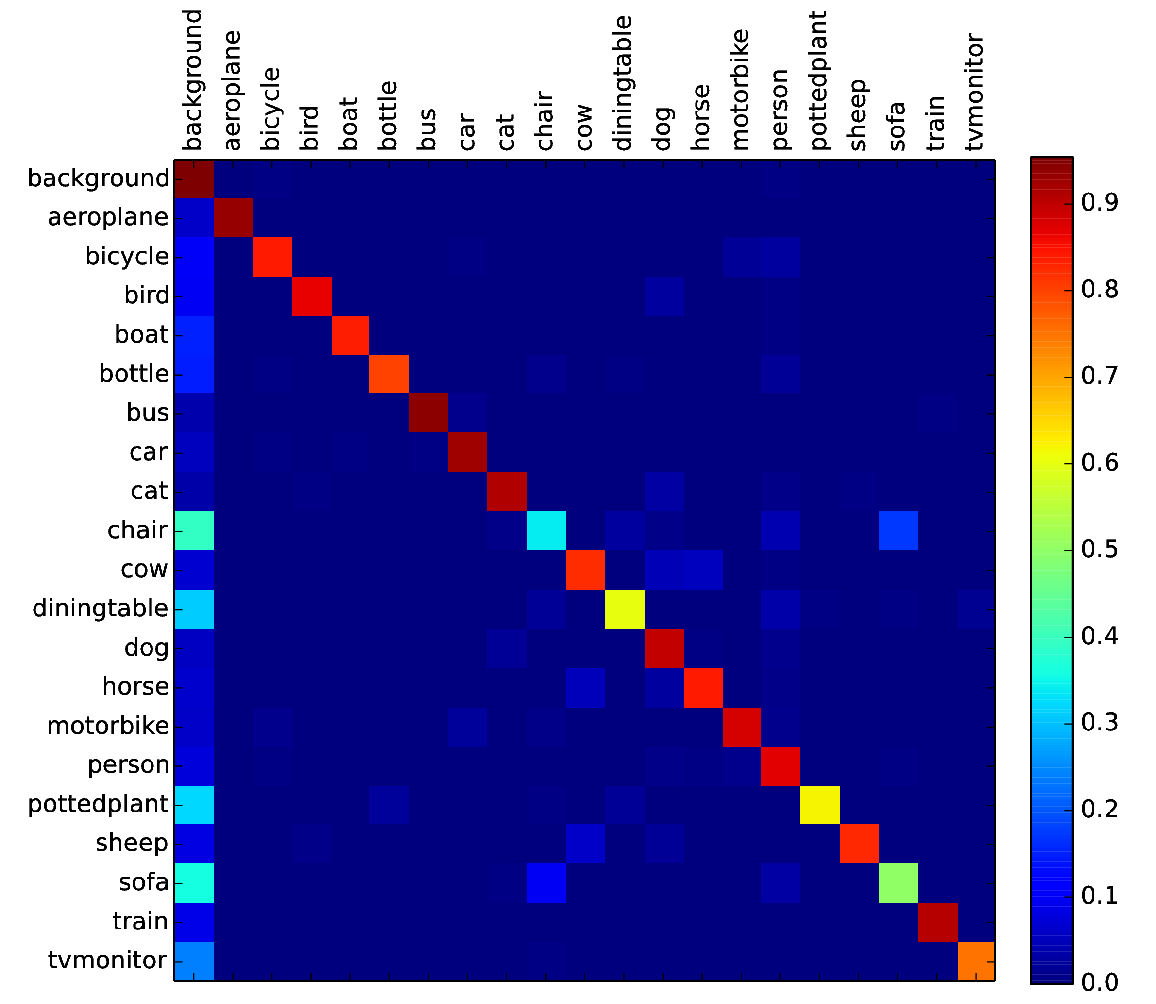
\includegraphics[width=0.5\textwidth]{image/result/confusion.pdf}
	\caption{镶嵌在文中的图像}
	\label{fig:confusion}
\end{wrapfigure}
论文主体是毕业论文的主要部分,必须言之成理,论据可靠,严格遵循本学科国际通行的学术规范。在写作上要注意结构合理、层次分明、重点突出,章节标题、公式图表符号必须规范统一。论文主体的内容根据不同学科有不同的特点,一般应包括以下几个方面: (1)毕业论文(设计)总体方案或选题的论证; (2)毕业论文(设计)各部分的设计实现,包括实验数据的获取、数据可行性及有效性的处理与分析、各部分的设计计算等; (3)对研究内容及成果的客观阐述,包括理论依据、创新见解、创造性成果及其改进与实际应用价值等; (4)论文主体的所有数据必须真实可靠,凡引用他人观点、方案、资料、数据等,无论曾否发表,无论是纸质或电子版,均应详加注释。自然科学论文应推理正确、结论清晰;人文和社会学科的论文应把握论点正确、论证充分、论据可靠,恰当运用系统分析和比较研究的方法进行模型或方案设计,注重实证研究和案例分析,根据分析结果提出建议和改进措施等。
\subsection{单张图像的插入}
\begin{figure}[h]
	\centering
	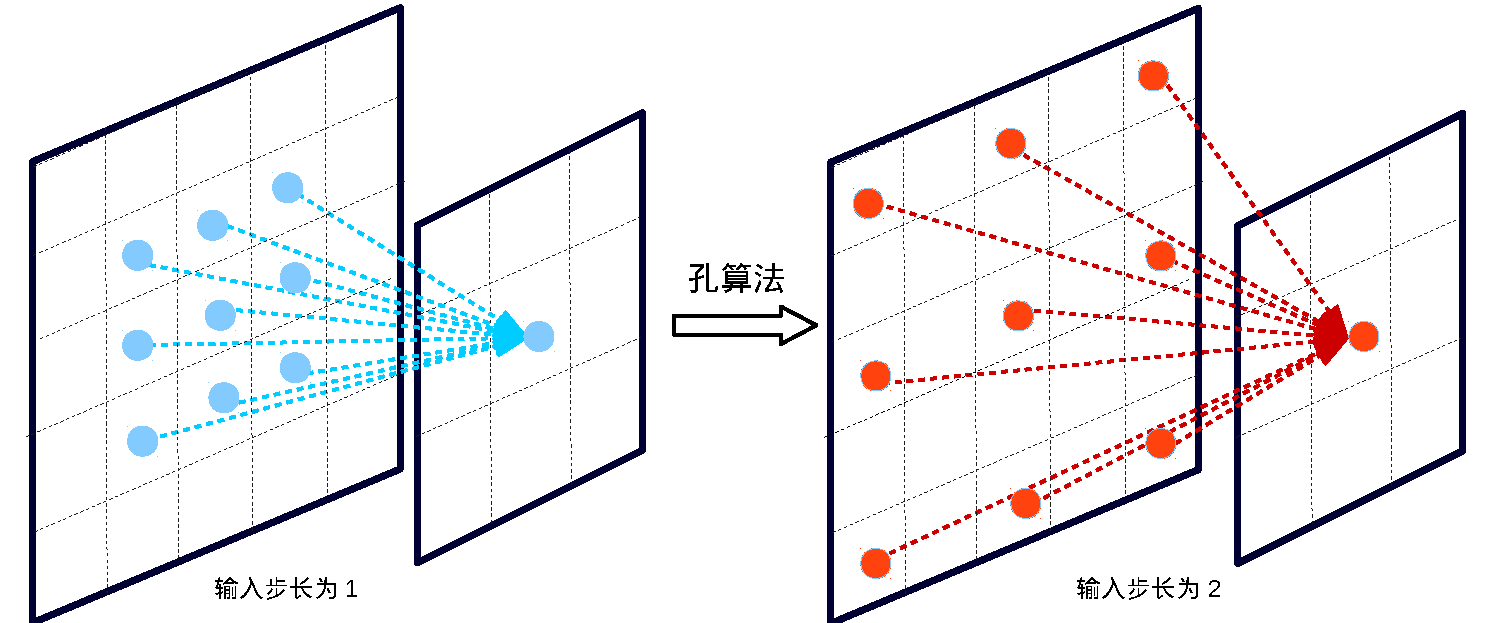
\includegraphics[width=0.5\textwidth]{image/illustration/hole.pdf}
	\caption{单张图像}
 	\label{fig:hole}
\end{figure}


\subsection{多张图像的并排插入}
\label{sub:多张图像的并排插入}
\begin{figure}[h!]%文中的Grid-LSTM模型做的语义图像分割的例子
	\centering
	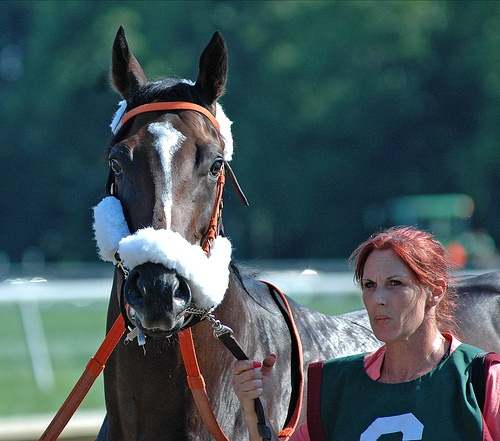
\includegraphics[width=.2\textwidth,height=.15\textwidth]{image/example/2007_000799.jpg}
	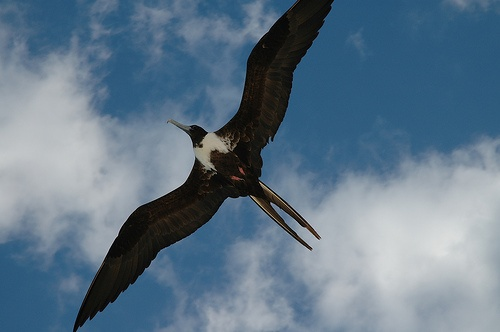
\includegraphics[width=.2\textwidth,height=.15\textwidth]{image/example/2007_002094.jpg}
	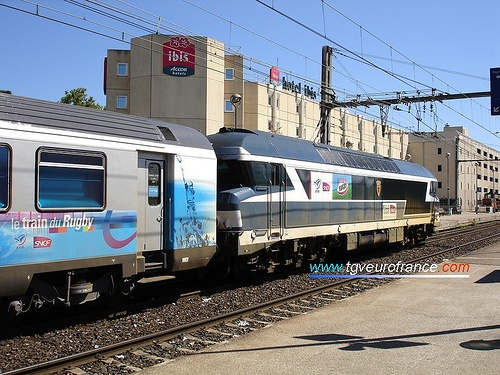
\includegraphics[width=.2\textwidth,height=.15\textwidth]{image/example/2007_004483.jpg}
	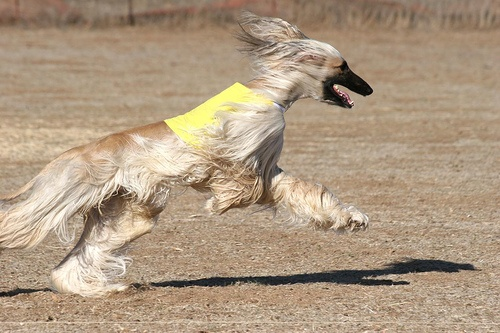
\includegraphics[width=.2\textwidth,height=.15\textwidth]{image/example/2007_003194.jpg}
	\\
	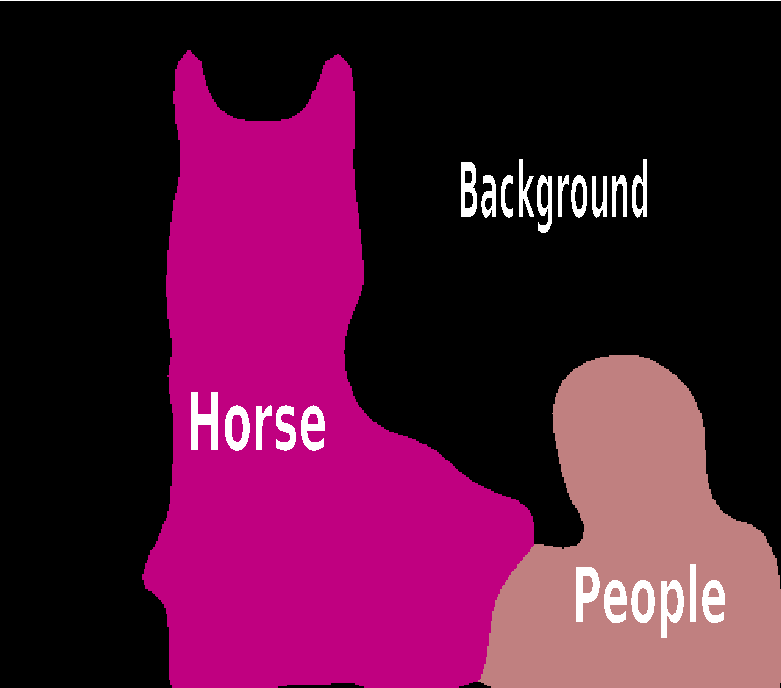
\includegraphics[width=.2\textwidth,height=.15\textwidth]{image/example/2007_000799.pdf}
	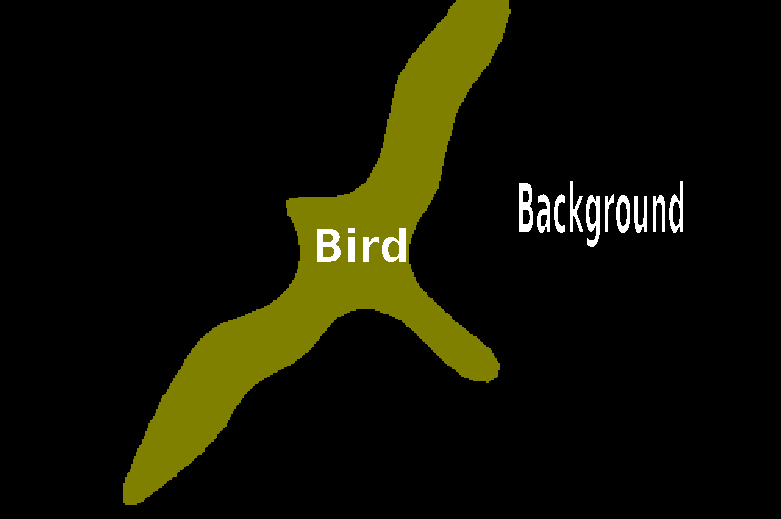
\includegraphics[width=.2\textwidth,height=.15\textwidth]{image/example/2007_002094.pdf}
	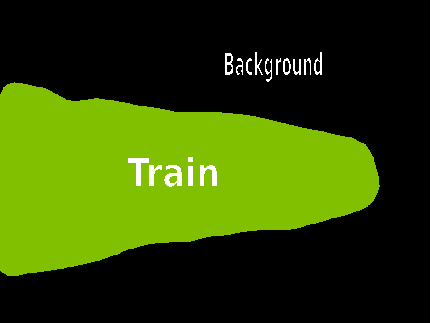
\includegraphics[width=.2\textwidth,height=.15\textwidth]{image/example/2007_004483.pdf}
	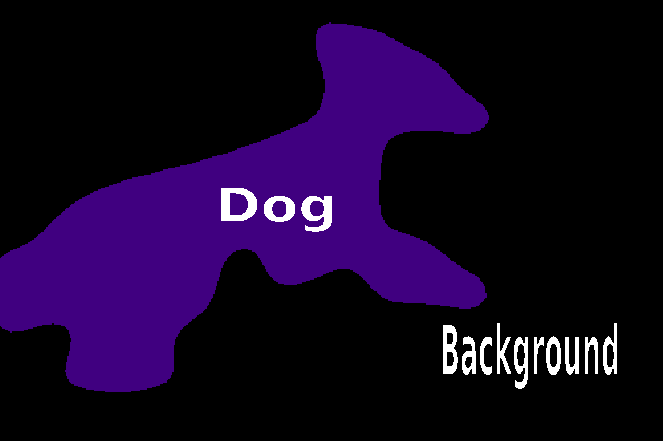
\includegraphics[width=.2\textwidth,height=.15\textwidth]{image/example/2007_003194.pdf}
	\caption{并排的多张图像}
	\label{fig:example1}
\end{figure}
\endinput

\begin{figure}[h]
\centering
	\makebox[0.11\textwidth]{\scriptsize 图像}
	\enspace
	\makebox[0.11\textwidth]{\scriptsize 真值}
	\enspace
	\makebox[0.11\textwidth]{\scriptsize CNN+5LSTM\textbf{1}}
	\enspace\thinspace
	\makebox[0.11\textwidth]{\scriptsize CNN+5LSTM\textbf{2}}
	\enspace\thinspace
	\makebox[0.11\textwidth]{\scriptsize CNN+5LSTM\textbf{3}}
	\enspace\thinspace
	\makebox[0.11\textwidth]{\scriptsize CNN+5LSTM\textbf{4}}
	\enspace\thinspace
	\makebox[0.11\textwidth]{\scriptsize CNN+5LSTM\textbf{5}}\\
	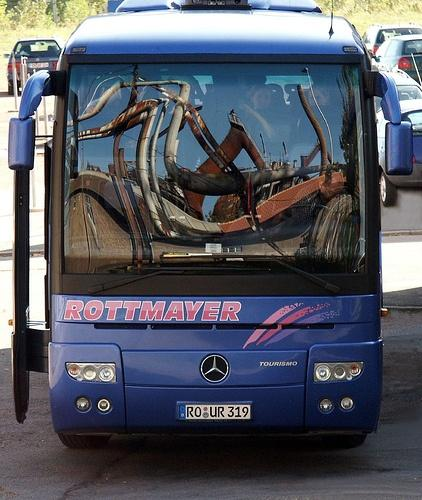
\includegraphics[width=0.11\textwidth]{image/improvement/2007_000663.jpg}
	\enspace\thinspace %\hfill
	
\includegraphics[width=0.11\textwidth]{image/improvement/2007_000663.png}
	\enspace\thinspace
	
\includegraphics[width=0.11\textwidth]{image/improvement/2007_000663_1.png}
	\enspace\thinspace
	
\includegraphics[width=0.11\textwidth]{image/improvement/2007_000663_2.png}
	\enspace\thinspace
	
\includegraphics[width=0.11\textwidth]{image/improvement/2007_000663_3.png}
	\enspace\thinspace
	
\includegraphics[width=0.11\textwidth]{image/improvement/2007_000663_4.png}
	\enspace\thinspace
	
\includegraphics[width=0.11\textwidth]{image/improvement/2007_000663_5.png}
	\enspace\thinspace
	\caption{并排的多张图像加各自的注解}
	\label{fig:improvement}
\end{figure}


\subsection{两列图像的插入}
\label{sec:complex}
\begin{figure}[h!] % image examples & compare
	\begin{subfigure}{0.55\textwidth}
		\makebox[0.18\textwidth]{\scriptsize Grid-5LSTM}
		\makebox[0.18\textwidth]{\scriptsize FCN-8s\cite{long2015fully}}
		\makebox[0.18\textwidth]{\scriptsize SDS\cite{hariharan2014simultaneous}}
		\makebox[0.18\textwidth]{\scriptsize 真值}
		\makebox[0.18\textwidth]{\scriptsize 图像} \\
		
\includegraphics[width=0.18\textwidth]{image/result/compare/my_horse.pdf}
		
\includegraphics[width=0.18\textwidth]{image/result/compare/fcn_horse.png}
		
\includegraphics[width=0.18\textwidth]{image/result/compare/sds_horse.png}
		
\includegraphics[width=0.18\textwidth]{image/result/compare/gt_horse.pdf}
		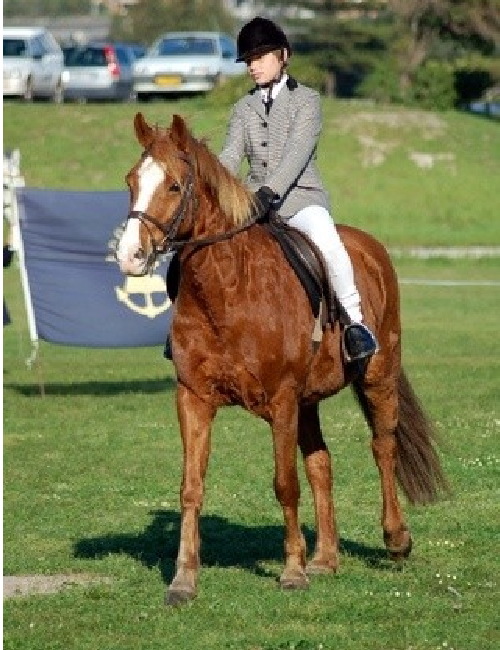
\includegraphics[width=0.18\textwidth]{image/result/compare/im_horse.pdf}
		\\
		
\includegraphics[width=0.18\textwidth]{image/result/compare/my_motor.png}
		
\includegraphics[width=0.18\textwidth]{image/result/compare/fcn_motor.png}
		
\includegraphics[width=0.18\textwidth]{image/result/compare/sds_motor.png}
		
\includegraphics[width=0.18\textwidth]{image/result/compare/2007_005173.png}
		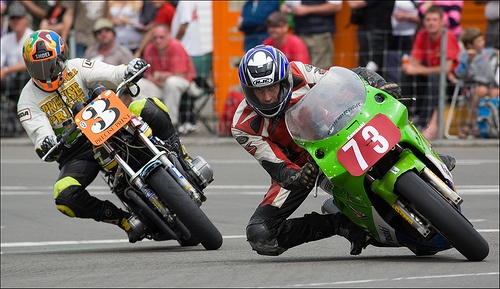
\includegraphics[width=0.18\textwidth]{image/result/compare/2007_005173.jpg}
		\\
		
\includegraphics[width=0.18\textwidth]{image/result/compare/my_sheep.pdf}
		
\includegraphics[width=0.18\textwidth]{image/result/compare/fcn_sheep.png}
		
\includegraphics[width=0.18\textwidth]{image/result/compare/sds_sheep.png}
		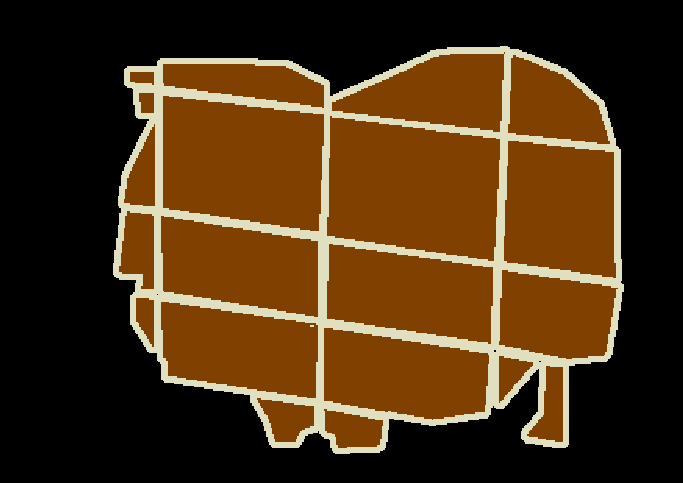
\includegraphics[width=0.18\textwidth]{image/result/compare/gt_sheep.pdf}
		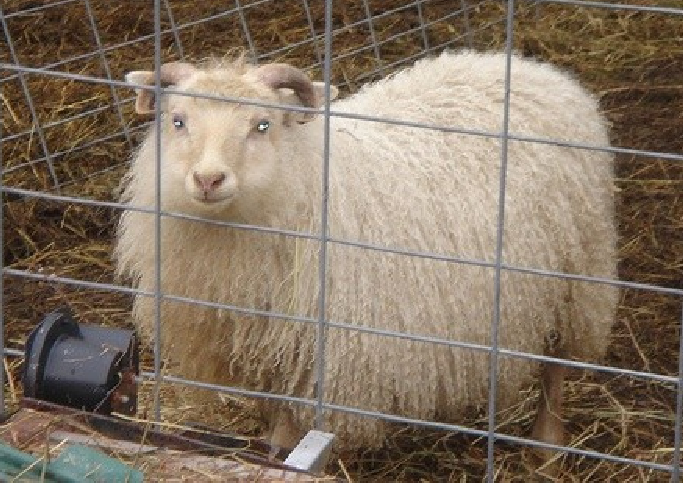
\includegraphics[width=0.18\textwidth]{image/result/compare/im_sheep.pdf}
		\\
		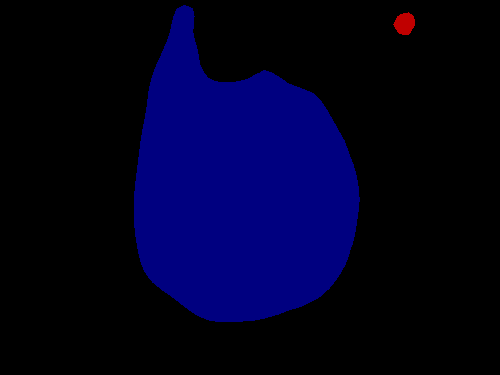
\includegraphics[width=0.18\textwidth]{image/result/compare/my_boat.png}
		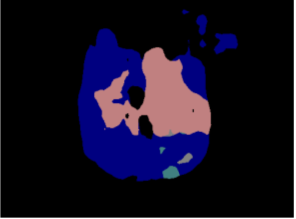
\includegraphics[width=0.18\textwidth]{image/result/compare/fcn_boat.png}
		
\includegraphics[width=0.18\textwidth]{image/result/compare/sds_boat.png}
		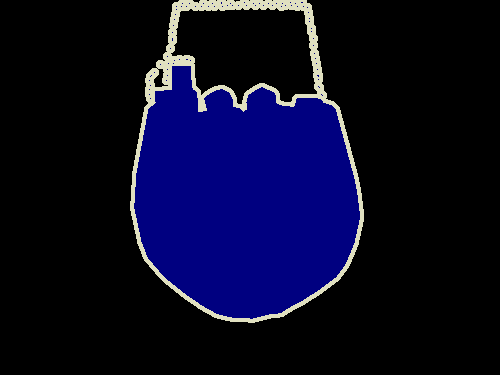
\includegraphics[width=0.18\textwidth]{image/result/compare/2007_004241.png}
		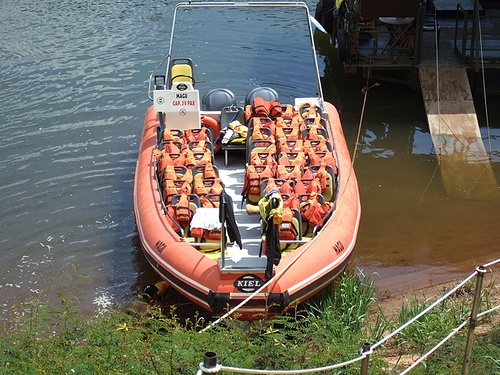
\includegraphics[width=0.18\textwidth]{image/result/compare/2007_004241.jpg}
		\caption{左边的图像}
		\label{fig:compare1}
	\end{subfigure}
	\begin{subfigure}{0.4\textwidth}
		\centering
%		\makebox[0.3\textwidth]{} \\
%		\makebox[0.3\textwidth]{} \\
		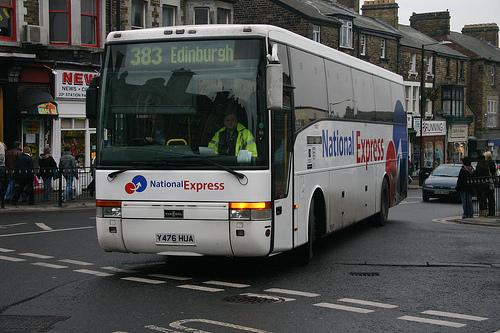
\includegraphics[width=0.25\textwidth]{image/result/compare/2010_005284.jpg}
		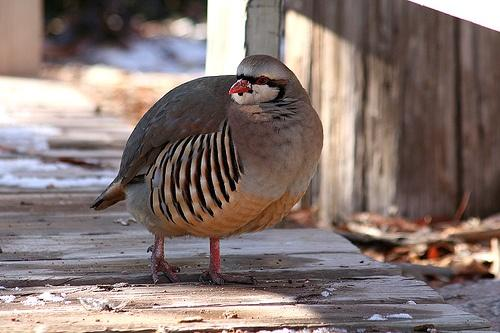
\includegraphics[width=0.25\textwidth]{image/result/compare/2007_003349.jpg}
		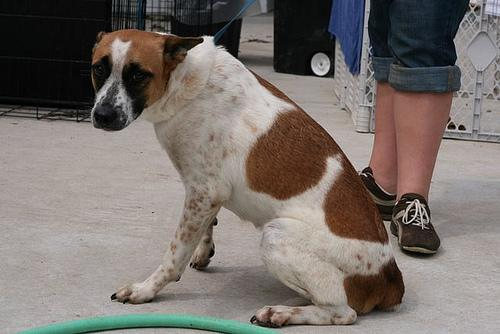
\includegraphics[width=0.25\textwidth]{image/result/compare/2009_004507.jpg} 
		\\
		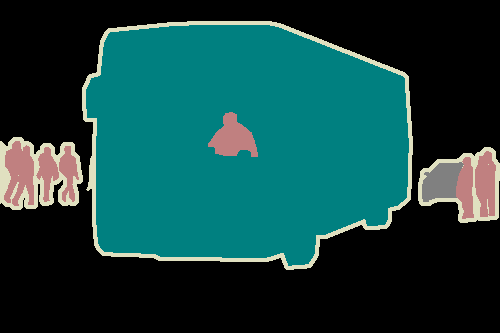
\includegraphics[width=0.25\textwidth]{image/result/compare/2010_005284.png}
		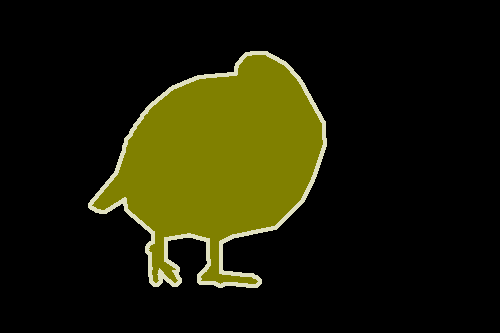
\includegraphics[width=0.25\textwidth]{image/result/compare/2007_003349.png}
		
\includegraphics[width=0.25\textwidth]{image/result/compare/2009_004507.png} \\
		
\includegraphics[width=0.25\textwidth]{image/result/compare/zoom_bus.png}
		
\includegraphics[width=0.25\textwidth]{image/result/compare/zoom_bird.png}
		
\includegraphics[width=0.25\textwidth]{image/result/compare/zoom_dog.png} \\
		
\includegraphics[width=0.25\textwidth]{image/result/compare/deeplab_bus.png}
		
\includegraphics[width=0.25\textwidth]{image/result/compare/deeplab_bird.png}
		
\includegraphics[width=0.25\textwidth]{image/result/compare/deeplab_dog.png} \\
		
\includegraphics[width=0.25\textwidth]{image/result/compare/my_bus.png}
		\includegraphics[width=0.25\textwidth]{image/result/compare/my_bird.png}
		\includegraphics[width=0.25\textwidth]{image/result/compare/my_dog.png} 
		\caption{右边的图像}
		\label{fig:compare2}
	\end{subfigure}
	\caption{复杂的两列对象的插入}
	\label{fig:complex}
\end{figure}


\clearpage

\section{表格的插入}
\label{sec:tables}
\begin{table}[h] %voc table result
	\centering
		\begin{tabular}{*{4}{c}}
			\toprule
	 		Method & Pixel Acc. & Mean Acc. & Mean Iu.\\
			\midrule
			Liu等人\cite{liu2011sift}  & 76.7 & - & -\\
		Tighe等人\cite{tighe2013finding}  & 78.6 & 39.2 & -\\
			FCN-16s\cite{long2015fully} & 85.2 & \textbf{51.7} & 39.5\\
			Deeplab-LargeFOV\cite{chen14semantic} & 85.6 & 51.2 & 39.7\\
			\midrule
			Grid-LSTM5 & \textbf{86.2} & 51.0 & \textbf{41.2}\\
			\bottomrule
		\end{tabular}
		\caption{典型的实验对比表格}		
		\label{tab:siftflow}
\end{table}

\begin{table}[h] %voc table result
\centering
	\resizebox{\textwidth}{!}{
	\begin{tabular}{c|*{20}{c}|c}
		\toprule
		Method & aero & bike & bird & boat & bottle & bus & car & cat & chair & cow & table & dog & horse & mbike & person & plant & shep & sofa & train & tv & mIoU.\\
		\midrule
		CNN				   & 72.6 & 29.6 & 70.2 & 53.1 & 65.1 & 81.0 & 74.3 & 79.8 & 25.0 & 64.8 & 47.8 & 69.5 & 66.2 & 65.2 & 74.2 & 42.1 & 69.6 & 38.8 & 74.4 & 58.6 & 62.5\\
		CNN+\textbf{1}LSTM & 71.5 & 30.6 & 70.5 & 53.8 & 64.9 & 82.4 & 77.1 & 79.5 & 25.1 & 65.8 & 47.8 & 71.5 & 64.6 & 67.0 & 74.0 & 43.9 & 69.6 & 38.6 & 74.9 & 59.4 & 63.0\\
		CNN+\textbf{2}LSTM & 76.1 & 32.6 & 72.1 & 57.0 & 65.3 & 83.6 & 75.4 & 81.7 & 24.7 & 69.3 & 47.5 & 72.3 & 68.9 & 69.5 & 74.7 & 41.5 & 69.8 & 38.3 & 77.8 & 62.1 & 64.3 \\
		CNN+\textbf{3}LSTM & 77.7 & 32.3 & 72.6 & 60.0 & 68.3 & 85.5 & 78.5 & 82.3 & 25.3 & 71.1 & 49.7 & 71.5 & 69.7 & 70.8 & 75.9 & 47.9 & 71.2 & 38.9 & 80.2 & 61.7 & 65.8 \\
		CNN+\textbf{4}LSTM & 79.1 & \textbf{33.7} & \textbf{73.6} & \textbf{62.0} & \textbf{70.4} & 85.5 & \textbf{80.9} & 83.7 & \textbf{24.1} & 70.7 & 45.7 & 73.7 & 69.6 & 72.1 & 75.6 & 47.2 & \textbf{76.0} & 37.3 & 80.5 & 62.2 & 66.4 \\
		CNN+\textbf{5}LSTM & \textbf{79.9} & 33.6 & \textbf{73.6} & 61.7 & 68.0 & \textbf{88.5} & \textbf{80.9} & \textbf{84.0} & 23.6 & \textbf{71.3} & \textbf{49.7} & \textbf{73.1} & \textbf{71.3} & \textbf{72.9} & \textbf{76.4} & \textbf{48.9} & 75.1 & \textbf{38.1} & \textbf{84.5} & \textbf{63.8} & \textbf{67.2} \\
		\midrule
		CNN+\textbf{5}LSTM$^\dag$ & 84.8 & 36.4 & 82.0 & 69.4 & 73.0 & 87.2 & 81.8 & 86.1 & 34.5 & 82.4 & 53.1 & 81.5 & 77.4 & 79.0 & 81.3 & 54.8 & 81.1 & 47.0 & 84.3 & 67.3 & 72.3 \\
		\bottomrule
	\end{tabular}}
	\caption{复杂一些的表格}		
	\label{tab:vocval}
\end{table}


\section{公式}
\label{sec:formula}
没有编号的公式
\begin{align*}
\begin{split}
	\label{eq:feedforward}
	\mybold{z}^{(l)} & = \mybold{W}^{(l)}\mybold{a}^{(l-1)} + \mybold{b}^{(l)} \\
	\mybold{a}^{(l)} & = f(\mybold{z}^{(l)})
\end{split}
\end{align*}
公式中含有中文
\begin{align}
	\begin{split}
	\mbox{像素准确率} &= \sum_{i=1}^{n_{cl}}n_{ii} / \sum_{i=1}^{n_{cl}}t_i \\
		\mbox{平均像素准确率} &= \frac{1}{n_{cl}} \sum_{i=1}^{n_{cl}}(n_{ii}/ t_i) \\
	\mbox{Mean IU} &= \frac{1}{n_{cl}} \sum_{i=1}^{n_{cl}}\frac{n_{ii}}{t_i + \sum_j^{n_{cl}} n_{ji} - n_{ii}}
	\end{split}
\end{align}
公式中含有矩阵
\begin{equation}
	\textbf{H} = \begin{bmatrix}
		I*\mybold{x}_i \\ \textbf{h}
	\end{bmatrix}
\end{equation}
每行后面都有编号的公式
\begin{align}
	\frac{\partial}{\partial W_{ij}^{(l)}} J(\mybold{W},\mybold{b};\mybold{x},y) &= \frac{\partial J(\mybold{W},\mybold{b};\mybold{x},y)}{\partial z_i^{(l+1)}}\cdot \frac{\partial z_i^{(l+1)}}{\partial W_{ij}^{(l)}} = \delta_i^{(l+1)}a_j^{(l)} \\
	\frac{\partial}{\partial b_i^{(l)}} J(\mybold{W},\mybold{b};\mybold{x},y) &= \frac{\partial J(\mybold{W},\mybold{b};\mybold{x},y)}{\partial z_i^{(l+1)}}\cdot \frac{\partial z_i^{(l+1)}}{\partial b_i^{(l)}} = \delta_i^{(l+1)}
\end{align}

\section{算法流程图}
\label{sec:algorithm}
\begin{algorithm}[h]
\KwIn{$m$个训练样本}
\lFor{$l=1$ \emph{\KwTo} $n_l$}{
初始化:$\Delta \mybold{W}^{(l)}=0$,$\Delta \mybold{b}^{(l)}=0$}
\ForEach{训练样本}{
	\lFor{$l=1$ \emph{\KwTo} $n_l-1$}{
	前向传播:$\mybold{z}^{(l+1)}=\mybold{W}^la^l+\mybold{b}^l$,$\mybold{a}^{(l+1)}=f(\mybold{z}^{(l+1)})$}
	输出误差计算:$\delta^{(n_l)} = \frac{\partial}{\partial \mybold{z}^{(n_l)}} J(\mybold{W},\mybold{b};\mybold{x},y)$\;
	\lFor{$l=n_l-1$ \emph{\KwTo} $1$}{
	后向传播:$\delta^{(l)} = \bigl((\mybold{W}^{(l)})^T \delta^{(l+1)}\bigr)f'(\mybold{z}^{(l)})$}
	\ForAll{层l}{
		计算梯度:$\nabla_{\mybold{W}^{(l)}}J(\mybold{W},\mybold{b};\mybold{x},y)=\delta^{(l+1)}(\mybold{a}^{(l)})^T$ \\
		\hspace{60pt}$\nabla_{\mybold{b}^{(l)}}J(\mybold{W},\mybold{b};\mybold{x},y)=\delta^{(l+1)}$\;
		累加梯度:$\Delta \mybold{W}^{(l)} \leftarrow \Delta \mybold{W}^{(l)} + \nabla_{\mybold{W}^{(l)}}J(\mybold{W},\mybold{b};\mybold{x},y)$; \\
		\hspace{60pt}$\Delta \mybold{b}^{(l)} \leftarrow \Delta \mybold{b}^{(l)} + \nabla_{\mybold{b}^{(l)}}J(\mybold{W},\mybold{b};\mybold{x},y)$\;
	}
}
\ForAll{层$l$}{
	更新权重:$\mybold{W}^{(l)} \leftarrow \mybold{W}^{(l)} - \alpha \biggl[\frac 1m \Delta \mybold{W}^{(l)}]$ \\
	\hspace{60pt} $\mybold{b}^{(l)} \leftarrow \mybold{b}^{(l)} - \alpha \biggl[\frac 1m \Delta \mybold{b}^{(l)}\biggr]$
}
\caption{梯度下降算法}
\label{algo:sgd}
\end{algorithm}

\section{例子与证明}
\subsection{例子}
\begin{eg}
  这是一个例子, 用以验证特殊环境的字体成功更改为楷体.
\end{eg}

\begin{proof}
  1. 大前提
  2. 小前提
  结论: 示例结论
\end{proof}

\section{其他的一些用法}
\label{sec:font}
这是一个列表
\begin{itemize}
	\item 引用文献\cite{long2015fully}
	\item 字体{\color{red}{变红}},\textbf{粗体}
	\item 索引前面的章节 \ref{sec:formula}、图像\ref{fig:complex}、表格\ref{tab:siftflow}
	\item 加脚注\footnote{http://cs231n.github.io/transfer-learning/}
\end{itemize}



        \chapter{研究方法}
\label{cha:experiment}

\section{应用功能设计}
\label{sec:app_design}
\begin{figure}[h]
	\centering
	\includegraphics[width=0.5\textwidth]{image/UML/ActivityDiagram.png}
	\caption{应用功能设计}
	\label{fig:app}
\end{figure}
\section{前端架构}
\label{sec:Front-end_architecture}

\section{界面设计}
\label{sec:UI}
阿里巴巴针对angular封装了对应的UI风格和许多实用的组件供开发者使用,让开发者不必花费过多的时间在UI的设计上面,让开发的周期变得更短。

使用方法:npm install ng-zorro-antd
\section{数据库设计}
\label{sec:database_design}
\begin{figure}[h]
	\centering
	\includegraphics[width=0.5\textwidth]{image/UML/ERDDiagram.png}
	\caption{数据库设计}
	\label{fig:database}
\end{figure}
\section{后端开发}
\label{sec:Backend_development }
dd
        %% chapter 4 dataset, network structure, experiment and result
\chapter{实验与结果}
\label{cha:experiment}


        \section{总结与展望}
\subsection*{总结与展望}
\frame{
   \footnotesize
	\begin{block}{工作总结}
	\begin{itemize}
		\item[\dag] 本文的模型结合了卷积网络的特征学习能力与长短记忆网络对整体局部建模的能力,相比于全卷积网络,大幅度地提高了了模型性能
		\item[\dag] 大量的对比实验与结果分析证明了模型的有效性 
	\end{itemize}
	\end{block}
	\vspace{-1em}
	\begin{block}{展望}
	\begin{itemize}
		\item[\dag] 模型性能:提高网络的深度来学习更高层次的特征,提高模型效果(He et al. ResNet, CVPR 2016)
		\item[\dag] 模型大小:通过裁剪网络冗余部分(Han et al. Deep Compression, ICLR 2016 Best Paper)或使用二值网络减少模型参数(Courbariaux et al. Binaryconnect, NIPS 2015)
		\item[\dag] 训练数据:使用无监督或弱监督的方式训练网络(Papandreou et al. Weakly-and semi-supervised learning, ICCV 2015)
	\end{itemize}
	\end{block}
}




        % 结语

    % 附录部分
    \backmatter
        % 参考文献. 因不需要纳入章节目录, 故放入附录部分
        % 实际上参考文献是属于论文主体部分
        \makereferences

        %%
% 致谢
% 谢辞应以简短的文字对课题研究与论文撰写过程中曾直接给予帮助的人员(例如指导教师、答疑教师及其他人员)表示对自己的谢意,这不仅是一种礼貌,也是对他人劳动的尊重,是治学者应当遵循的学术规范。内容限一页。
% modifier: 黄俊杰
% update date: 2017-04-15
%%

\chapter{致谢}

	四年时间转眼即逝,青涩而美好的本科生活快告一段落了。回首这段时间,我不仅学习到了很多知识和技能,而且提高了分析和解决问题的能力与养成了一定的科学素养。虽然走过了一些弯路,但更加坚定我后来选择学术研究的道路,实在是获益良多。这一切与老师的教诲和同学们的帮助是分不开的,在此对他们表达诚挚的谢意。

	首先要感谢的是我的指导老师林倞教授。我作为一名本科生,缺少学术研究经验,不能很好地弄清所研究问题的重点、难点和热点,也很难分析自己的工作所能够达到的层次。林老师对整个研究领域有很好的理解,以其渊博的知识和敏锐的洞察力给了我非常有帮助的方向性指导。他严谨的治学态度与辛勤的工作方式也是我学习的榜样,在此向林老师致以崇高的敬意和衷心的感谢。

	最后我要感谢我的家人,正是他们的无私的奉献和支持,我才有了不断拼搏的信息的勇气,才能取得现在的成果。

\vskip 108pt
\begin{flushright}
	陈冠英\makebox[1cm]{} \\
\today
\end{flushright}

    % 致谢

        % 附录
    \appendix
        % \chapter{参考文献}

% \begin{figure}[h!]
% \centering
% 		\makebox[0.16\textwidth]{\scriptsize 图像}
% 		\makebox[0.16\textwidth]{\scriptsize 真值}
% 		\makebox[0.16\textwidth]{\scriptsize Grid-5LSTM1}
% 		\makebox[0.16\textwidth]{\scriptsize Grid-5LSTM3}
% 		\makebox[0.16\textwidth]{\scriptsize Grid-5LSTM5} \\
% 		\includegraphics[width=0.16\textwidth]{image/appendix1/2007_000042.jpg}
% 		\includegraphics[width=0.16\textwidth]{image/appendix1/2007_000042.png}
% 		\includegraphics[width=0.16\textwidth]{image/appendix1/1/2007_000042.png} 
% 		\includegraphics[width=0.16\textwidth]{image/appendix1/3/2007_000042.png}
% 		\includegraphics[width=0.16\textwidth]{image/appendix1/5/2007_000042.png} \\

% 		\includegraphics[width=0.16\textwidth]{image/appendix1/2011_003256.jpg}
% 		\includegraphics[width=0.16\textwidth]{image/appendix1/2011_003256.png}
% 		\includegraphics[width=0.16\textwidth]{image/appendix1/1/2011_003256.png} 
% 		\includegraphics[width=0.16\textwidth]{image/appendix1/3/2011_003256.png}
% 		\includegraphics[width=0.16\textwidth]{image/appendix1/5/2011_003256.png} \\
% 		\includegraphics[width=0.16\textwidth]{image/appendix1/2011_001159.jpg}
% 		\includegraphics[width=0.16\textwidth]{image/appendix1/2011_001159.png}
% 		\includegraphics[width=0.16\textwidth]{image/appendix1/1/2011_001159.png} 
% 		\includegraphics[width=0.16\textwidth]{image/appendix1/3/2011_001159.png}
% 		\includegraphics[width=0.16\textwidth]{image/appendix1/5/2011_001159.png} \\
% 		\includegraphics[width=0.16\textwidth]{image/appendix1/2011_000813.jpg}
% 		\includegraphics[width=0.16\textwidth]{image/appendix1/2011_000813.png}
% 		\includegraphics[width=0.16\textwidth]{image/appendix1/1/2011_000813.png} 
% 		\includegraphics[width=0.16\textwidth]{image/appendix1/3/2011_000813.png}
% 		\includegraphics[width=0.16\textwidth]{image/appendix1/5/2011_000813.png} \\
% 		\includegraphics[width=0.16\textwidth]{image/appendix1/2011_003145.jpg}
% 		\includegraphics[width=0.16\textwidth]{image/appendix1/2011_003145.png}
% 		\includegraphics[width=0.16\textwidth]{image/appendix1/1/2011_003145.png} 
% 		\includegraphics[width=0.16\textwidth]{image/appendix1/3/2011_003145.png}
% 		\includegraphics[width=0.16\textwidth]{image/appendix1/5/2011_003145.png} \\
% 		\includegraphics[width=0.16\textwidth]{image/appendix1/2009_004579.jpg}
% 		\includegraphics[width=0.16\textwidth]{image/appendix1/2009_004579.png}
% 		\includegraphics[width=0.16\textwidth]{image/appendix1/1/2009_004579.png} 
% 		\includegraphics[width=0.16\textwidth]{image/appendix1/3/2009_004579.png}
% 		\includegraphics[width=0.16\textwidth]{image/appendix1/5/2009_004579.png} \\
% \color[rgb]{0.9,0.9,0.9}\bfseries
% \begin{tabular}{*{7}{>{\centering\arraybackslash}p{0.10\textwidth}}}
% 	\hline
% 	\cellcolor[rgb]{0,0,0}  背景&\cellcolor[rgb]{0.5020,0,0} 飞机 &\cellcolor[rgb]{0,0.5020,0} 自行车 &\cellcolor[rgb]{0.5020,0.5020,0} 鸟 &\cellcolor[rgb]{0,0,0.5020} 船   &\cellcolor[rgb]{0.5020,0,0.5020} 瓶子 &\cellcolor[rgb]{0,0.5020,0.5020} 大巴
% 	\\
% 	\hline
% 	\cellcolor[rgb]{0.5020,0.5020,0.5020} 汽车 & \cellcolor[rgb]{0.2510,0,0} 猫 &\cellcolor[rgb]{0.7529,0,0} 椅子 &\cellcolor[rgb]{0.2510,0.5020,0} 牛 &\cellcolor[rgb]{0.7529,0.5020,0} 桌子 &\cellcolor[rgb]{0.2510,0,0.5020} 狗 &\cellcolor[rgb]{0.7529,0,0.5020} 马 \\
% 	\hline
% 	\cellcolor[rgb]{0.2510,0.5020,0.5020} 摩托车 &\cellcolor[rgb]{0.7529,0.5020,0.5020} 人   &\cellcolor[rgb]{0,0.2510,0} 盆栽   &\cellcolor[rgb]{0.5020,0.2510,0} 羊 &\cellcolor[rgb]{0,0.7529,0} 沙发 &\cellcolor[rgb]{0.5020,0.7529,0} 火车 &\cellcolor[rgb]{0,0.2510,0.5020} 电视 \\
% 	\hline
% \end{tabular}

% \caption{一个配有彩色表格的插图}
% \end{figure}

% \endinput
\begin{thebibliography}{123456}
	\bibitem {Gao}Gao C Y,Cui Y B,Heng-TaocL I.A Study of the Application of Basic Path Testing Method[J].Journal of Kaifeng University,2012.
	\bibitem {XU}徐晖,冯永兵,肖传娥,等.基于SQL的数据存储和查询[J].山西电子技术,2001,29(3):15-17
	\bibitem {Yang}杨芙清,梅宏,李克勤.软件复用与软件构件技术[J].电子学报,1999,27(2):68-75.
	\bibitem {Zorro}Ant Design,Ant Design of Angular NG-ZORRO[EB/OL],https://ng.ant.design, 2018-4-20.
	\bibitem {Angular}Angular,Angular中文网[EB/OL],https://www.angular.cn/, 2018-4-20.
	\bibitem {Sequelize}Jonas Zhang,Sequelize Docs 中文版http://docs.sequelizejs.com/, 2018-2-23.
	\bibitem {multer}npm,multer,https://www.npmjs.com/package/multer, 2018-4-20.
	\bibitem {Nodejs}Nodejs,Nodejs中文文档,http://nodejs.cn/, 2018-4-20.
	\bibitem {jm}广发证券互联网金融技术团队.揭秘Angular 2[M].北京:电子工业出版社,2017:20-37.
	\bibitem {Chen}陈文海.软件测试管理工具的研究与实现[D].中国科学院研究生院(软件研究所),2003.
	\bibitem {yuan}袁勤勇.软件工程领域的经典教材——张海藩的《软件工程导论(第5版)》[J].计算机教育,2008,(5):96-97.
	\bibitem {rahayu}Rahayu J A.free,web,hosting,affiliate,unikom,MI,php,mysql[J].
	\bibitem {ng}Ari Lerner; Felipe Coury; Nate Murray; Carlos Taborda.Angular权威教程[M].北京:人民邮电出版社,2017:17-30.
\end{thebibliography}

    \makeGrade      % 成绩评定记录表
\end{document}

